\scanpage{10}
\uline{Exercice} \handwritten{4}.\handwritten{10}.\handwritten{6} . Soient \(S\) un \(\underline{U}\)-site dont la topologie est moins fine que la canonique , \(\underline{\unsure{\deleted{S}\handwritten{M}|\handwritten{M}|\handwritten{\mathscr{M}}}}\) une partie de \(\mathrm{Fl}(S)\) possédant les propriétés suivantes :

 a) Les morphismes de \(\underline{M}\) sont quarrables (I \handwritten{10}.\handwritten{3}) et \(\underline{\unsure{\deleted{S}M|\mathbb{M}|\deleted{M}S}}\) est stable par changement de base.

 b) \(\underline{\deleted{S}M}\) contient les flèches identiques et est stable par composition .
% The composite glyph in b repeats the unresolved typed glyph in a; see the first-occurrence doubt and notation entry.

 c) Une flèche \(u:X\to Y\) telle qu'il existe une famille couvrante \(Y_i\to Y\) , avec les \(X\times_Y Y_i\to Y_i\) dans \(\underline{M}\) , est elle-même dans \(\underline{M}\) .

 d) Pour tout objet \(X\) , toute famille couvrante de \(X\) est raffinée par une famille couvrante \((f_i:X_i\to X)\) où les \(f_i\) sont dans \(\underline{M}\).

Pour tout objet \(X\) , \deleted{considérons le site}\inserted{notons} \(S(X)\) (``petit site de \(X\)'')%
\handwritten{\begin{tikzpicture}[x=1em,y=1em,baseline=-.25ex]
\draw[line width=.35pt] (0,0) -- (.32,.81);
\draw[line width=.35pt] (.35,.88) ellipse (.10 and .12);
\end{tikzpicture}}%
\reversemarginpar\margin{%
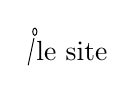
\begin{tikzpicture}[x=1em,y=1em,baseline=(label.base)]
\handwritten{\draw[line width=.35pt] (0,-.18) -- (.21,.80);
\draw[line width=.35pt] (.24,1.03) ellipse (.075 and .13);}
\node[anchor=base west,inner sep=0pt] (label) at (.28,0) {\inserted{le site}};
\end{tikzpicture}}\normalmarginpar
\deleted{dont la catégorie sous-jacente est}\inserted{constitué par} la sous-catégorie pleine de \(S/X\) formée des objets dont le morphisme structural est dans \(\underline{M}\) , munie de la topologie induite par celle de \(S\) (III \handwritten{3}.\handwritten{1}).

1) Montrer que les familles couvrantes \((f_i:X_i\to X)_{i\varepsilon I}\) où les \(f_i\) sont dans \(\underline{M}\) forment une prétopologie sur \(S\) (II \handwritten{1}.\handwritten{3}) qui engendre la topologie de \(S\) .

2) Pour toute flèche \(u:X\to Y\) de \(S\) , montrer que le foncteur changement de base par \(u\) est un foncteur continu (III \handwritten{1}.\handwritten{1}) de \(S(Y)\) dans \(S(X)\) . \unsure{\deleted{e}O|\deleted{o}O|\(\mathbb{O}\)}n notera
\[
S(u)^{\handwritten{*}}:S(Y)^{\handwritten{\sim}}\to S(X)^{\handwritten{\sim}}
\]
le foncteur correspondant entre les catégorie\handwritten{s} de faisceaux (III \handwritten{1}.\handwritten{2},iv)).

3) Définir une équivalence entre le topos \(S^{\handwritten{\sim}}\) et la catégorie des systèmes
\[
(F_X)\ (X\varepsilon\operatorname{ob}S)\quad,\quad(\handwritten{\varphi_u})\ (u\varepsilon\mathrm{Fl}\ S)
\]
formés d'objets \(F_X\varepsilon\operatorname{ob}S(X)^{\handwritten{\sim}}\) , et pour toute flèche \(u:X\to Y\) dans \(S\) , d'un morphisme \(\handwritten{\varphi}_u:S(u)^{\handwritten{*}}(F_Y)\to F_X\) , ces systèmes
% archive sheet number: 9
